%!TEX root = ../main.tex

\section{Operator Space Details}
\label{sec:appendix_operator_space}

In this section, we provide the complete definitions of all 31 operators supported by \sys (Section~\ref{subsec:operator_space}), along with analyses of operator pipeline length distribution and operator type distribution across datasets.

\subsection{Complete Operator Definitions}
\label{subsec:appendix_operator_definitions}

\begin{table*}[t]
  \centering
  \caption{\bf Taxonomy of supported data preparation operators by functional type.}
  \vspace{-0.6em}
  \label{tbl:operator_space_type}

  \small
  \setlength{\tabcolsep}{6pt}
  \renewcommand{\arraystretch}{1.12}

  \resizebox{\textwidth}{!}{
    \begin{tabular}{|l||l|}
      \hline
      \textbf{Operator Type} & \textbf{Operators} \\
      \hline \hline

      \textbf{Data Cleaning} &
      \texttt{MissingValueImputation},
      \texttt{Deduplicate},
      \texttt{ErrorDetection},
      \texttt{OutlierDetection},
      \texttt{DropNA} \\
      \hline

      \textbf{Value Normalization} &
      \texttt{ValueTransform},
      \texttt{StandardizeDatetime},
      \texttt{CastType} \\
      \hline

      \textbf{Schema Editing} &
      \texttt{RenameColumn},
      \texttt{SplitColumn},
      \texttt{AddNewColumn},
      \texttt{DropColumn},
      \texttt{Concatenate},
      \texttt{SelectColumn},
      \texttt{Subtitle} \\
      \hline

      \textbf{Row Selection} &
      \texttt{Filter},
      \texttt{Sort},
      \texttt{TopK} \\
      \hline

      \textbf{Aggregation} &
      \texttt{GroupBy},
      \texttt{Count},
      \texttt{CalculateStatistic} \\
      \hline

      \textbf{Table Combination} &
      \texttt{Join},
      \texttt{Union},
      \texttt{Append} \\
      \hline

      \textbf{Table Reshaping} &
      \texttt{Pivot},
      \texttt{Stack},
      \texttt{WideToLong},
      \texttt{Transpose},
      \texttt{Explode} \\
      \hline

      \textbf{Program Synthesis} &
      \texttt{ExeCode} \\
      \hline
    \end{tabular}
  }
\end{table*}


As outlined in Table~\ref{tbl:operator_space}, the operators are categorized into four groups: Data Cleaning, Column Transformation, Table Transformation, and Other. We detail the functionality and parameters for each operator below.

\stitle{Operators for Data Cleaning.}
These operators focus on improving data quality by handling errors, missing values, and inconsistencies.

(1) $\mathtt{StandardizeString}$.
    This function standardizes the string format within a specific column. It accepts two arguments: {\small\texttt{column}}, representing the target column name, and {\small\texttt{func}}, a lambda function defining the transformation logic. For example, to remove whitespace and convert the \term{City} column to title case, we set {\small\texttt{column}} to \term{City} and {\small\texttt{func}} to {\small\texttt{lambda x: x.strip().title()}}.

(2) $\mathtt{ErrorDetection}$.
    This function identifies erroneous values based on specific logic. It takes {\small\texttt{column}} and {\small\texttt{func}} as arguments, where {\small\texttt{func}} returns a boolean indicating validity. For instance, to detect invalid email addresses, {\small\texttt{func}} could be a regex match function {\small\texttt{lambda x: not re.match(r"[\^{}@]+@[\^{}@]+\.[\^{}@]+", x)}}.

(3) $\mathtt{DropNA}$.
    This function removes rows containing missing values. It requires {\small\texttt{subset}}, a list of columns to inspect for null values, and {\small\texttt{how}}, which specifies the condition (\eg {\small\texttt{'any'}} or {\small\texttt{'all'}}). For example, to drop rows where both \term{Revenue} and \term{Cost} are missing, we set {\small\texttt{subset}} to {\small\texttt{['Revenue', 'Cost']}} and {\small\texttt{how}} to {\small\texttt{'all'}}.

(4) $\mathtt{MVI}$ (Missing Value Imputation).
    This function fills missing values using a specified strategy. It takes {\small\texttt{column}} and {\small\texttt{mode}} as arguments. The {\small\texttt{mode}} can be a statistical method (\eg {\small\texttt{'mean'}}, {\small\texttt{'median'}}) or a constant value. For example, to fill missing values in the \term{Age} column with the average age, we set {\small\texttt{column}} to \term{Age} and {\small\texttt{mode}} to {\small\texttt{'mean'}}.

(5) $\mathtt{OutlierDetection}$.
    This function handles statistical outliers. It accepts {\small\texttt{column}}, {\small\texttt{mode}} (\eg {\small\texttt{'z-score'}}, {\small\texttt{'iqr'}}), and {\small\texttt{action}} (\eg {\small\texttt{'clip'}}, {\small\texttt{'drop'}}). For instance, to cap values in the \term{Price} column that exceed 3 standard deviations, we set {\small\texttt{mode}} to {\small\texttt{'z-score'}} and {\small\texttt{action}} to {\small\texttt{'clip'}}.

(6) $\mathtt{StandardizeDatetime}$.
    This function converts a column to a standard datetime object. It requires {\small\texttt{column}} and {\small\texttt{date-format}}. For example, to parse dates like ``2023/12/25'' in the \term{Date} column, we set {\small\texttt{date-format}} to {\small\texttt{"\%Y/\%m/\%d"}}.

(7) $\mathtt{Deduplicate}$.
    This function removes duplicate rows. It takes {\small\texttt{subset}} (columns to consider for identifying duplicates) and {\small\texttt{keep}} (which duplicate to retain, \eg {\small\texttt{'first'}}, {\small\texttt{'last'}}, or {\small\texttt{'none'}}).

\stitle{Operators for Column Transformation.}
These operators modify the schema by adding, removing, or restructuring columns.

(1) $\mathtt{AddNewColumn}$.
    This function creates a new column based on row-wise calculation. It takes a single argument {\small\texttt{func}}, a lambda function accepting a row dictionary. For example, to create a \term{Profit} column, we use {\small\texttt{lambda row: row['Revenue'] - row['Cost']}}.

(2) $\mathtt{Cast}$.
    This function converts the data type of a column. Its arguments are {\small\texttt{column}} and {\small\texttt{dtype}} (\eg {\small\texttt{'int'}}, {\small\texttt{'float'}}, {\small\texttt{'str'}}). For example, to convert a \term{Year} column stored as text to integers, we set {\small\texttt{dtype}} to {\small\texttt{'int'}}.

(3) $\mathtt{Explode}$.
    This function transforms each element of a list-like string into a row, replicating index values. It takes {\small\texttt{column}} and {\small\texttt{split-comma}} (the separator). As shown in Example~\ref{exam:agentic_tree_based_reasoning}, to split ``Sci-Fi/Action'' in the \term{Genre} column into separate rows, we set {\small\texttt{split-comma}} to {\small\texttt{'/'}}.

(4) $\mathtt{RenameColumn}$.
    This function renames existing columns. It accepts {\small\texttt{rename-map}}, a dictionary mapping old names to new names. \eg {\small\texttt{\{'Yr': 'Year', 'Pop': 'Population'\}}}.

(5) $\mathtt{DropColumn}$.
    This function removes columns from the table. It takes {\small\texttt{drop-columns}}, a list of column names to delete.

(6) $\mathtt{SplitColumn}$.
    This function splits a single column into multiple columns based on a pattern. It requires {\small\texttt{src-column}} and {\small\texttt{func}}. For example, to extract the numeric rating from a string ``8.5/10'', we set {\small\texttt{func}} to {\small\texttt{lambda x: x.split('/')[0]}}.

(7) $\mathtt{Concatenate}$.
    This function combines multiple columns into one string column. It takes {\small\texttt{columns}} (list of source columns) and {\small\texttt{func}} (formatting logic). For example, to combine \term{First} and \term{Last} names, {\small\texttt{func}} could be {\small\texttt{lambda x: f"\{x['First']\} \{x['Last']\}"}}.

\stitle{Operators for Table Transformation.}
These operators restructure the table shape or aggregate data.

(1) $\mathtt{Join}$.
    This function merges two tables. Arguments include {\small\texttt{left}} and {\small\texttt{right}} (table names), {\small\texttt{on}} (join keys), and {\small\texttt{how}} (type of join: {\small\texttt{'inner'}}, {\small\texttt{'left'}}, {\small\texttt{'outer'}}).

(2) $\mathtt{Union}$ / $\mathtt{Append}$.
    These functions combine tables vertically. $\mathtt{Union}$ takes a list of {\small\texttt{tables}} and a {\small\texttt{how}} parameter (\eg set logic), while $\mathtt{Append}$ specifically adds {\small\texttt{appended-table}} to the end of {\small\texttt{src-table}}.

(3) $\mathtt{Pivot}$.
    This function reshapes data from long to wide format. It requires {\small\texttt{index}}, {\small\texttt{columns}} (keys to become new headers), and {\small\texttt{values}}. For example, pivoting a sales table to show months as columns.

(4) $\mathtt{Transpose}$.
    This function swaps rows and columns of the table. It takes no parameters.

(5) $\mathtt{Stack}$ / $\mathtt{WideToLong}$.
    These functions reshape data from wide to long format. $\mathtt{Stack}$ takes {\small\texttt{id-vars}} (columns to keep) and {\small\texttt{value-vars}} (columns to unpivot). $\mathtt{WideToLong}$ handles more complex patterns with suffix extraction defined by {\small\texttt{subnames}}, {\small\texttt{i}}, {\small\texttt{j}}, and {\small\texttt{sep}}.

(6) $\mathtt{Subtitle}$.
    This function is used to handle hierarchical headers often found in spreadsheets. It takes {\small\texttt{title}} to identify the main header row and propagates it to sub-headers.

(7) $\mathtt{Sort}$.
    This function sorts the table rows. It takes {\small\texttt{by}} (column names) and {\small\texttt{ascending}} (boolean).

(8) $\mathtt{GroupBy}$.
    This function groups data and applies aggregation. It requires {\small\texttt{by}} (grouping columns) and {\small\texttt{agg}} (a dictionary mapping columns to functions, \eg {\small\texttt{\{'Profit': 'mean'\}}}).

(9) $\mathtt{TopK}$.
    This function retains the top-$k$ rows based on a specific order. It takes the integer argument {\small\texttt{k}}.

(10) $\mathtt{Filter}$.
    This function filters rows based on a condition. It takes {\small\texttt{func}}, a lambda function returning a boolean for each row. \eg {\small\texttt{lambda row: row['Year'] > 2000}}.

(11) $\mathtt{SelectColumn}$.
    This function selects a subset of columns to keep, discarding the rest. It takes {\small\texttt{columns}} as a list.

(12) $\mathtt{Count}$.
    This function counts the number of records, optionally grouped by unique values. It takes {\small\texttt{table-name}}.

(13) $\mathtt{CalculateStatistic}$.
    This function computes statistics across tables or complex aggregations. It takes {\small\texttt{tables}}, {\small\texttt{var-name}}, and {\small\texttt{func}}.

\stitle{Other Operators.}
These operators handle special cases and flow control.

(1) $\mathtt{CodeGeneration}$.
    This function allows the agent to generate arbitrary Python code for tasks not covered by the predefined operators. It takes {\small\texttt{tables}} and the generated {\small\texttt{code}} string. This ensures \sys can handle long-tail requirements.

(2) $\mathtt{Terminate}$.
    This operator signals the end of the reasoning process. It takes {\small\texttt{output-tables}} to specify the final result to be returned to the user.

In total, we define \textbf{31} distinct operators, providing comprehensive coverage for diverse data cleaning and transformation tasks.

\subsection{Operator Pipeline Length Distribution}
\label{subsec:appendix_pipeline_length}

\begin{figure}[t]
    \centering
    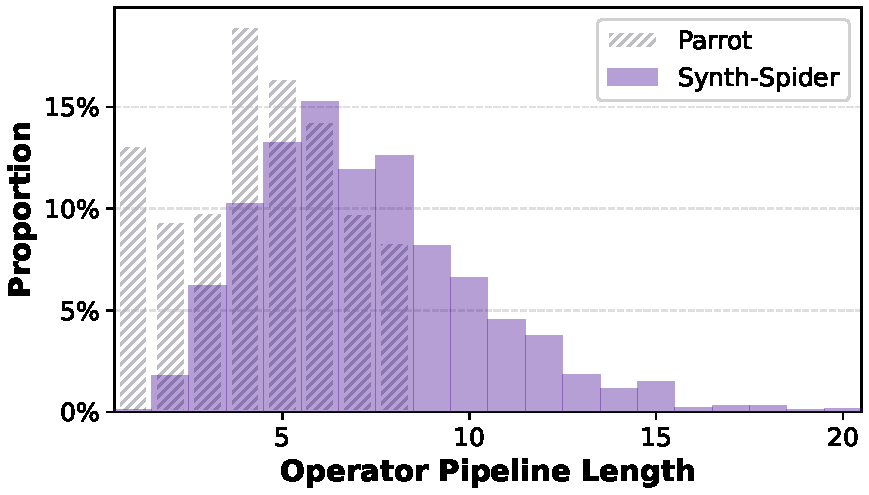
\includegraphics[width=0.95\columnwidth]{plots/plot/op_len_distribution.pdf}
    \vspace{-1em} 
    \caption{Operator Pipeline Length Distribution.}
    \label{fig:op_len_distribution}
    \vspace{-0.5em}
    % \vspace{-1em}
\end{figure}

Figure~\ref{fig:op_len_distribution} shows the distribution of operator pipeline lengths across Synth-Spider, Synth-Bird, and Parrot. Synth-Spider and Synth-Bird share a similar pipeline length distribution, with the majority of pipelines containing 3--7 operators. In contrast, Parrot exhibits a noticeably different distribution, with pipelines tending to be shorter and less varied in length. This difference in pipeline length distribution partially explains the transfer performance gap observed in Exp-\ref{exp:data_effectiveness}.

\subsection{Operator Type Distribution}
\label{subsec:appendix_operator_distribution}

\begin{figure}[t]
    \centering
    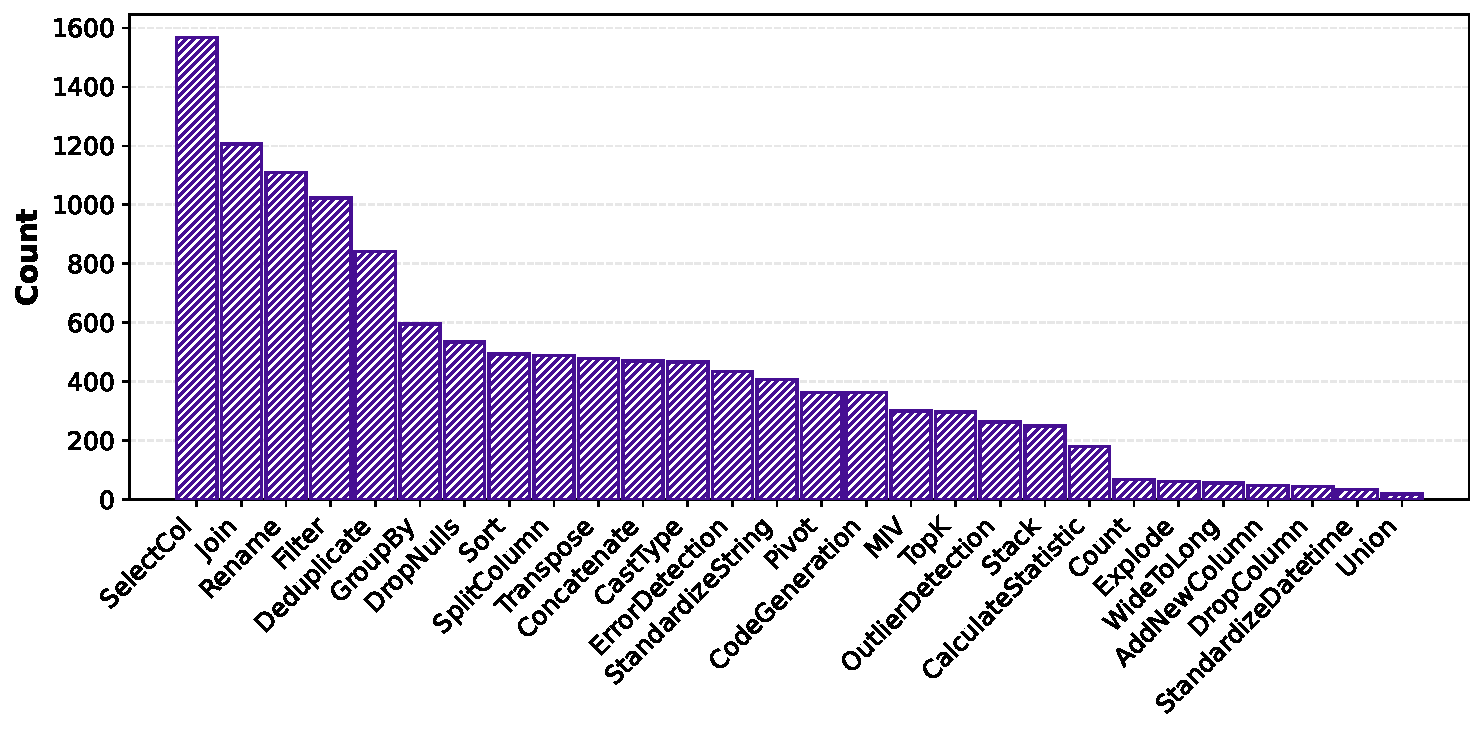
\includegraphics[width=0.99\columnwidth]{appendix/figures/fig/op_type_count_spider.pdf}
    \vspace{-1em} 
    \caption{Operator Count Distribution on Synth-Spider.}
    \label{fig:op_type_count_spider}
    % \vspace{-1em}
\end{figure}
\begin{figure}[t]
    \centering
    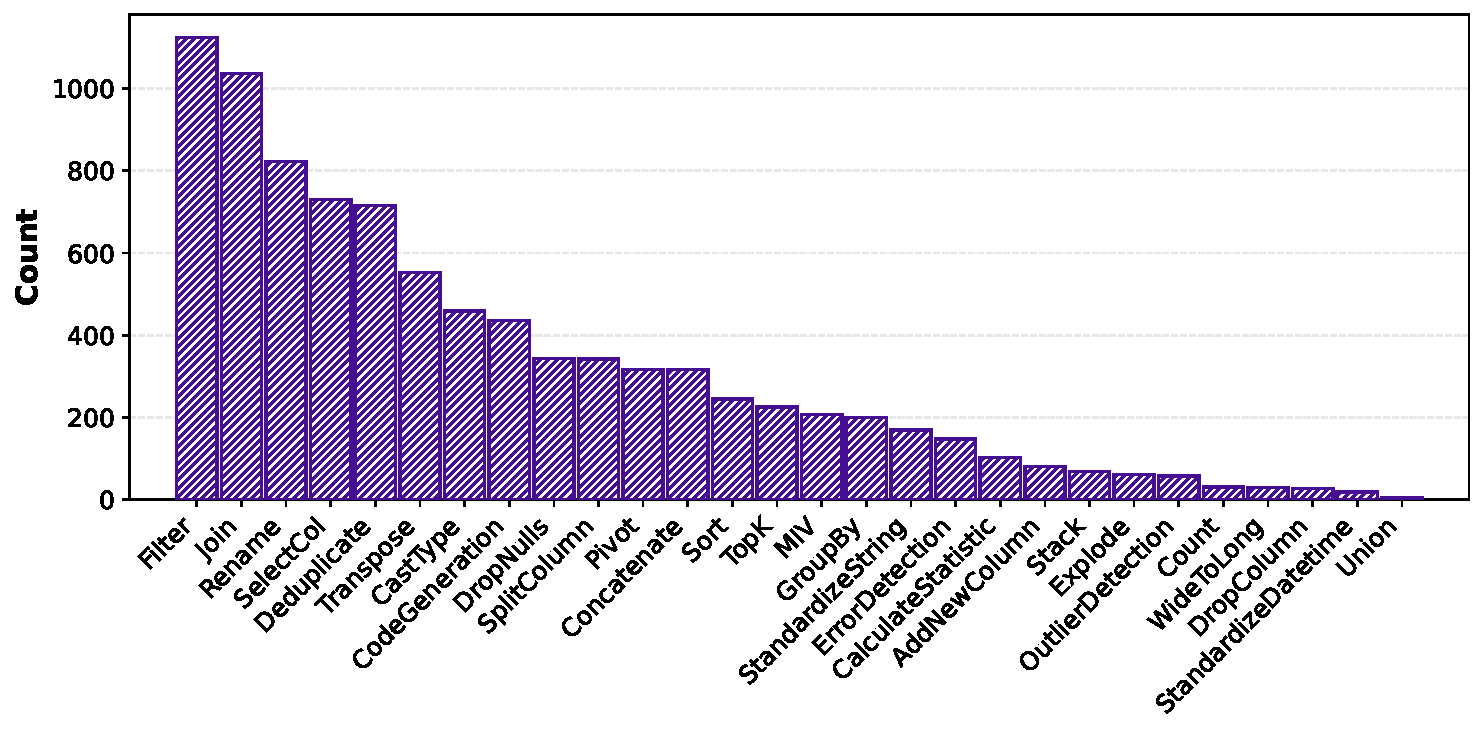
\includegraphics[width=0.99\columnwidth]{appendix/figures/fig/op_type_count_bird.pdf}
    \vspace{-1em} 
    \caption{Operator Count Distribution on Synth-Bird.}
    \label{fig:op_type_count_bird}
    % \vspace{-1em}
\end{figure}

Figures~\ref{fig:op_type_count_spider} and~\ref{fig:op_type_count_bird} show the operator type distributions on Synth-Spider and Synth-Bird, respectively. As discussed in Exp-\ref{exp:data_effectiveness}, the operator-type distribution shift is the primary factor explaining transfer performance, rather than pipeline length distribution. We provide a finer-grained analysis of operator coverage and compositional diversity:

\stitle{Operator Coverage.}
Our Synth-Spider dataset provides broader operator coverage than Parrot in three aspects. First, as shown in Table~\ref{tbl:datasets}, Synth-Spider supports 14 additional types of operators compared with Parrot, including commonly used data cleaning operations such as Missing Value Imputation, as well as common schema editing operations such as Concatenation. Second, our operators support function arguments, enabling more customized data preparation operations. For example, \texttt{AddNewColumn} can take a lambda expression as an argument to define a customized mapping from source columns to the newly created column. Third, we include highly flexible data preparation operators such as \texttt{ExeCode}. When a data preparation requirement cannot be covered by the currently defined operator space, \texttt{ExeCode} allows the model to complete the operation by writing executable code.

\stitle{Operator Distribution Similarity.}
The unigram Jensen-Shannon Divergence (JSD) between Synth-Spider and Synth-Bird is only 0.025, with a cosine similarity of 0.952, indicating nearly identical distributions. In contrast, the JSD between Synth-Bird and Parrot is 0.264 (\textbf{10.6$\times$ larger}), and the bigram and trigram JSDs reach 0.660 and 0.886 respectively, indicating nearly disjoint compositional patterns.

\stitle{Compositional Diversity.}
Synth-Spider and Synth-Bird produce 496 and 417 unique bigrams (2,875 and 1,947 unique trigrams), while Parrot yields only 189 and 758 respectively. Synth-Spider and Synth-Bird also exhibit higher cross-category bigram ratios (0.799/0.765 vs.\ Parrot's 0.708), meaning their operator combinations span more diverse functional categories. Synth-Spider's top-5 and top-10 bigram concentration ratios are also lower than Parrot's (0.226 and 0.326 vs.\ 0.248 and 0.361), indicating that its operator distribution is less dominated by a few frequent patterns.
